\documentclass[11pt]{article}

\usepackage[utf8]{inputenc}
\usepackage[T1]{fontenc}
\usepackage[margin=1in]{geometry}
\usepackage{amsmath, amssymb, amsthm}
\usepackage{mathtools}
\usepackage{hyperref}
\usepackage{xcolor}
\usepackage{enumitem}
\usepackage{microtype}
\usepackage{parskip}
\usepackage{graphicx}
\graphicspath{{Figures/}{../paper/theory/figures/}{../benchmarks/plots/TE_demonstration/}{../benchmarks/plots/TE_demonstration/panels/}}
\usepackage{booktabs}
\usepackage{subcaption}
\usepackage{natbib}

\newtheorem{theorem}{Theorem}
\newtheorem{corollary}[theorem]{Corollary}
\newtheorem{lemma}[theorem]{Lemma}
\newtheorem{remark}[theorem]{Remark}
\newtheorem{assumption}{Assumption}

\newcommand{\PP}{\mathbb{P}}
\newcommand{\EE}{\mathbb{E}}
\newcommand{\Var}{\mathrm{Var}}
\newcommand{\Cov}{\mathrm{Cov}}
\newcommand{\Ino}{\mathcal{I}}
\newcommand{\NLL}{\mathrm{NLL}}

\hypersetup{
  colorlinks=true,
  linkcolor=blue!60!black,
  urlcolor=blue!60!black,
  citecolor=blue!60!black
}

\newcommand{\LUKE}[1]{{\color{blue}#1}}

\setlist{itemsep=2pt, parsep=2pt, topsep=4pt}

\title{Causal Foundation Models (Title will change)}
\begin{document}
\maketitle

%======================================================================
\section{Introduction}

\LUKE{
\section{Background and related work}

\subsection{Structural causal model and interventions}
\label{sec:scm-outcomes}
We work with an observational dataset $\mathcal{D}_{\text{obs}} = \{(X_i, T_i, Y_i)\}_{i=1}^n$, where each row records a unit's covariates $X_i \in \mathbb{R}^d$, the treatment it actually received $T_i \in \{0,1\}$, and the outcome observed under that treatment, $Y_i \in \mathbb{R}$. 

We assume $\mathcal{D}_{\text{obs}}$ is generated by a structural causal model (SCM) $\psi = (G, f, p_\varepsilon)$ over $\{X, T, Y\}$: $G$ a directed graph, $f = \{f_V\}$ structural equations shared across all units, $p_\varepsilon$ the exogenous noise distribution. Each row of $\mathcal{D}_{\text{obs}}$ is one sample $\varepsilon_i \sim p_\varepsilon$ propagated through $f$. 

An intervention $\text{do}(T=t)$ under SCMs sets the treatment to value $t$ and severs its dependence on its normal causal parents, while leaving every other structural equation untouched. This defines the potential outcome:
$$Y^{\text{do}(t)}(x,\varepsilon) = f_Y\big(x, t, \mathrm{pa}_{-T}(\psi;x,\varepsilon), \varepsilon_Y\big), \quad t\in\{0,1\}.$$
where $\mathrm{pa}_{-T}(\psi; x, \varepsilon)$ denotes the values of $Y$'s graph-parents other than $T$, propagated through $\psi$.

We assume $Y^{\text{do}(0)}$ and $Y^{\text{do}(1)}$ share the same noise draw $\varepsilon$, so they are \textit{coupled} rather than independent — this coupling is what a paired observation carries and a single-outcome observation does not. Because the generating mechanism is fully specified for any SCM used as a synthetic data source, this coupling lets us sample both potential outcomes of a synthetic unit together:

\begin{assumption}[Paired-outcome sampling]
\label{ass:regularity}
For every $x$ in the support of $X$, $\EE_{p_\varepsilon}[Y_{\mathrm{do}(t)}(x,\varepsilon)^2] < \infty$ for $t \in \{0, 1\}$, and the SCM admits paired-outcome sampling: a single draw $\varepsilon \sim p_\varepsilon$ yields both $Y_{\mathrm{do}(0)}(x, \varepsilon)$ and $Y_{\mathrm{do}(1)}(x, \varepsilon)$.
\end{assumption}

The conditional average treatment effect (CATE) at covariate value $x$ is
$$\tau(x) := \mathbb{E}\big[Y^{\text{do}(1)} - Y^{\text{do}(0)} \mid X = x\big],$$
and the average treatment effect (ATE) is its average over the covariate population, $\mathbb{E}_X[\tau(X)]$.

\textcolor{red}{general version of MALC can be introduced here, or beginning of section 3. We specify how MALC is used/adjusted inline when we need it} \textcolor{orange}{No need for the MALC here, we can discuss why that is in a meeting once we complete the first draft.}


\subsection{Prior-data fitted networks for Bayesian inference}
\label{sec:pfn}
We define Bayesian prediction as the task of computing the posterior predictive distribution (PPD), $p(y \mid x, \mathcal{D})$, for a query $x$ given an observed dataset $\mathcal{D}$:
\begin{equation}
p(y \mid x, \mathcal{D}) = \int_{\Theta} p(y \mid x, \theta)\, p(\theta \mid \mathcal{D})\, d\theta
\end{equation}
where predictions are averaged over a hypothesis space $\Theta$, weighted by the posterior belief $p(\theta \mid \mathcal{D}) \propto p(\mathcal{D} \mid \theta) p(\theta)$.

Instead of evaluating this integral anew for every dataset — intractable outside conjugate special cases — Prior-Data Fitted Networks (PFNs) amortize the computation: a neural network $q_\phi$ is trained once, offline, on synthetic $(\theta, \mathcal{D})$ pairs sampled from the prior $p(\theta)$, directly approximating the PPD. At inference time, a real dataset $\mathcal{D}_{\text{real}}$ is provided as context, and the network outputs an approximation to $p(y \mid x, \mathcal{D}_{\text{real}})$ in a single forward pass without gradient updates.

\subsection{Causal foundation models}
\label{sec:cfm}
Causal foundation models (CFMs) apply the PFN paradigm to causal effect estimation. In this setting, the hypothesis space consists of structural causal models (SCMs) $\psi \sim p(\psi)$. Given covariates $x$ and an observational dataset $\mathcal{D}_{\text{obs}}$, a CFM parameterised by $\phi$ produces an amortized posterior predictive distribution
\begin{equation}
q_\phi\big(Y \mid \mathcal{D}_{\text{obs}}, x, \text{do}(t)\big)
\end{equation}
for each intervention value $t \in \{0, 1\}$.

\textcolor{red}{DoPFN, UWYK, CausalPFN, CausalFM}
}



%======================================================================
\section{Methodology}
\label{sec:joint-head}

Current causal foundation models \citep{REF} train a single-outcome head on $(T_i, Y_i)$ pairs, using only the outcome under the treatment assigned to each unit. This convention discards half of the information relevant to estimation and limits the effective capacity of the model. We replace the single-outcome head with one that outputs the joint density over the paired potential outcomes; two consequences follow. Section~\ref{sec:performance} establishes that the joint objective halves the asymptotic mean-squared error of every marginal density and, by linearity, of the CATE and ATE estimators themselves. Section~\ref{sec:info-gain} shows that the joint density recovers dependence structure between $Y_{\mathrm{do}(0)}$ and $Y_{\mathrm{do}(1)}$ that no pair of marginals can express, enabling distributional inference over CATE and ATE that a marginal head can produce only conservatively. 

%----------------------------------------------------------------------
\subsection{Statistical efficiency of the joint objective}
\label{sec:performance}

For each query covariate $X$ with observational context
$\mathcal{D}_{\mathrm{obs}} = \{(X_i, T_i, Y_i)\}_{i=1}^{N}$, the joint head predicts a density $f(y_0, y_1 \mid X, \mathcal{D}_{\mathrm{obs}})$ on $\mathbb{R}^2$. The training loss is the negative log-density against paired labels drawn from the SCM prior,
\begin{equation}
  \mathcal{L}(y_0^\star, y_1^\star \mid X, \mathcal{D}_{\mathrm{obs}})
  \;=\;
  -\log f(y_0^\star, y_1^\star \mid X, \mathcal{D}_{\mathrm{obs}}),
  \label{eq:nll}
\end{equation}
averaged over queries in a batch. Positivity of $f$ on all of $\mathbb{R}^2$ is required for the loss to remain finite. We enforce it by combining a bounded interior $K \times K$ grid on $\mathcal{I} = [-1,1]^2$ with Gaussian tails along the four extended-axis and four diagonal directions, producing a nine-region mixture. This construction requires $K^2 + 9 + 4$ trainable parameters per query, and at the values of $K$ used by marginal-only head models the quadratic dependence would explode the computational cost. We therefore train at $K=\sqrt{J}$, where $J$ is the baseline marginal-only model's grid. Naively reducing the per-dimension resolution, however, shrinks the
model's representational capacity, uniformly degrading its estimation quality across both point and distributional metrics.  

We overcome this issue by applying MALC~\citep{} at inference. MALC is a mixture-of-log-concave estimator over uniformly binned data that
produces both point and density estimations. It recovers the true values on wider grids—smaller $K$—up to a small bounded error, provided the per-bin probabilities are themselves estimated with sufficient accuracy. Because the head is trained under
that objective, $K=\sqrt{J}$ suffices to preserve the model's representational capacity, and the joint head's parameter count then matches that of a marginal-only, preserving the computational cost. Appendices~\ref{app:head-spec} and~\ref{app:malc} detail the construction of the joint head and the MALC procedure (base class, mixture order-selection criterion, per-query inference cost), respectively.

With computational cost matched and representational capacity addressed, we examine the statistical efficiency of the joint objective. Lemma~\ref{lem:sufficiency} establishes that the joint head is strictly more efficient than the marginal one: the objective in~\eqref{eq:nll} retains at least all the information available to the marginal objective. \\

% Having established that the joint head can be designed to be no more expensive than a marginal one, we show in
% Lemma~\ref{lem:sufficiency} that it is also statistically strictly more efficient. The objective in~\eqref{eq:nll} contains at a minimum all the information available to the marginal objective; equivalently, the marginal's information is a subset of the joint's. \\

\begin{lemma}
\label{lem:sufficiency}
Let $Z_i^{\mathrm{R}} \coloneqq (X_i, Y_{\mathrm{do}(0)}(x_i, \varepsilon_i),
Y_{\mathrm{do}(1)}(x_i, \varepsilon_i))$ denote the per-unit observation
under the joint objective and
$Z_i^{\mathrm{U}} \coloneqq (X_i, T_i, Y_{T_i}(x_i, \varepsilon_i))$
the per-unit observation under the marginal objective, with $T_i$
drawn from any distribution on $\{0, 1\}$ independent of
$\varepsilon_i$. Then $Z^{\mathrm{U}}$ is a randomised function of
$Z^{\mathrm{R}}$: sampling $T$ from the same distribution and setting
$Z^{\mathrm{U}} = (X, T, Y_T)$ recovers the law of the single-outcome
observation from that of the paired one. Consequently any parameter
of the joint law
$\PP^\star(Y_{\mathrm{do}(0)}, Y_{\mathrm{do}(1)} \mid X)$ estimable
from $Z^{\mathrm{U}}$ is estimable from $Z^{\mathrm{R}}$ at least as
well.
\end{lemma}

Because the treatment, $T_i$, is randomly assigned, the marginal observation contains information about $Y_{\mathrm{do}(t)}$ only for the $t$ selected by $T_i$; the joint observation, by contrast, contains information about both potential outcomes at every unit. The Fisher information the marginal objective discards therefore depends on the distribution of $T_i$.  Theorem~\ref{thm:efficiency} shows that this loss propagates, via the Cram\'er--Rao bound, to the mean-squared error of every marginal density and, by linearity, to the CATE estimator itself. \\


\begin{theorem}
\label{thm:efficiency}
Let $T_i \sim \mathrm{Bernoulli}(\pi)$ with $\pi \in (0, 1)$, write
$\pi_1 = \pi$ and $\pi_0 = 1 - \pi$, and assume standard MLE
regularity. For every query $x$:
\begin{enumerate}[label=(\roman*), leftmargin=1.8em]
  \item for each $t \in \{0, 1\}$, the marginal density estimators
    satisfy
    \begin{equation}
      \lim_{N \to \infty} N \cdot
        \EE\!\bigl[(\hat p_{\mathrm{U}}(y \mid x, t) - p^\star(y \mid x, t))^2\bigr]
      \;=\;
      \frac{1}{\pi_t} \cdot
      \lim_{N \to \infty} N \cdot
        \EE\!\bigl[(\hat p_{\mathrm{R}}(y \mid x, t) - p^\star(y \mid x, t))^2\bigr];
      \label{eq:marg-ratio}
    \end{equation}
  \item the CATE estimator
    $\hat\tau(x) = \hat\mu_1(x) - \hat\mu_0(x)$ satisfies
    \begin{equation}
      \lim_{N \to \infty}
        \frac{\EE[(\hat\tau^{\,\mathrm{U}}(x) - \tau(x))^2]}
             {\EE[(\hat\tau^{\,\mathrm{R}}(x) - \tau(x))^2]}
      \;=\;
      \frac{1}{2\pi(1-\pi)}.
      \label{eq:R-bound}
    \end{equation}
\end{enumerate}
\end{theorem} 

The ratio in~\eqref{eq:R-bound} rescales the whole limiting error distribution. The Corollary~\ref{cor:stability} records this second consequence: the joint objective is more stable across problems, not merely more accurate on average. \\

\begin{corollary}
\label{cor:stability}
Under the same conditions,
\[
  \lim_{N \to \infty}
    \frac{\mathrm{Std}_{\mathrm{SCMs}}(\sqrt{\mathrm{PEHE}}^{\,\mathrm{R}})}
         {\mathrm{Std}_{\mathrm{SCMs}}(\sqrt{\mathrm{PEHE}}^{\,\mathrm{U}})}
  \;=\; \sqrt{2\pi(1-\pi)}.
\]
\end{corollary} 

Proofs of Lemma~\ref{lem:sufficiency}, Theorem~\ref{thm:efficiency} and
Corollary~\ref{cor:stability} are given in Appendix~\ref{app:proofs}. 

The results are asymptotic in $N$ and do not depend on the covariate dimension
$d$, though larger $d$ requires larger $N$ before the limit becomes
informative. Three conditions can nevertheless prevent the theory from
materialising in practice. First, the Cram\'er--Rao bound governs variance
under maximum likelihood, so training under a non-MLE proper-scoring loss may
preserve the qualitative ordering while losing the predicted magnitude of the
improvement. Second, the ordering relies on the estimator converging to the
true marginal density; if the joint parameterisation approximates the marginal strictly worse than the marginal-only one, the ordering can flip.
Third, the predicted improvement is a reduction in variance, and the theory
assumes the asymptotic regime in which bias does not dominate the error; when
it does, the improvement may not be visible in practice. We therefore verify the theory empirically in Section~\ref{sec:results},
reporting controlled simulations that measure whether the improvement
materialises, the rate of asymptotic convergence, and how the sample complexity
scales with $d$.

%----------------------------------------------------------------------
\subsection{Distributional inference for CATE and ATE}
\label{sec:info-gain}

The primary purpose of any model, including tabular foundation models, is to
provide information to the user for a better-informed decision. For users
interested merely in the observational distribution, models such as
TabPFN~\cite{TABPFN} deliver sufficient information about the variable of interest by
reporting both its density and a scalar point estimate. Existing CFMs, however,
fall short of this standard for users interested in the interventional
distribution, and report only a limited view: some provide a scalar CATE estimate together with a distribution over responses under each treatment~\cite{...}, while others provide a scalar CATE with a distribution over the treatment effect but no response information~\cite{...}. To our knowledge, no
existing method delivers the response and CATE distributions
simultaneously, and no existing method delivers an ATE distribution at all. A decision maker using a CFM, however, generally requires all three: the response densities support outcome decisions (e.g., whether a treated unit's outcome exceeds a clinical or economic threshold), while the CATE and ATE densities support the treatment decision itself (e.g., whether to intervene at all). One might argue that a point-wise CATE estimate combined with the marginal densities already provides sufficient information for this decision; however, same point estimate and confidence interval can arise from different shapes of uncertainty that call for different actions. For example, a near-uniform effect density and a bimodal density with two contrasting (negative and positive) modes can yield identical point estimates and confidence intervals: the uniform density
indicates that no action can be preferred over another, whereas the bimodal density indicates that with domain knowledge one may favour one mode over the other.

To recover the missing distributional information, one might attempt to reconstruct a CATE distribution from the marginals, but this is possible only under an independence assumption between $Y_{\mathrm{do}(0)}$ and $Y_{\mathrm{do}(1)}$, which is generally false, and discarding the coupling yields spurious treatment-effect values. The joint head resolves this gap and simultaneously refines the marginal response distribution that current models already provide; it therefore both improves what existing models report and delivers the additional information decision makers require.

Sections~\ref{sec:cate-malc} and~\ref{sec:ate-barycenter} describe how the per-unit CATE density and the population-level ATE density are recovered from the joint head's output.

\subsubsection{Per-unit CATE distribution via MALC}
\label{sec:cate-malc}

The joint head produces a discrete distribution on a $K \times K$
grid with mass $p_{ij}$ at bin centre $(y_0^i,\, y_1^j)$. MALC fits
a continuous joint density $\hat p(y_0, y_1)$ to these bin masses
as a mixture of log-concave components. The per-unit CATE density
then follows by the change of variables
$(Y_0, Y_1) \mapsto (Y_0, \tau)$ with
$\tau := Y_{\mathrm{do}(1)} - Y_{\mathrm{do}(0)}$, marginalising
out $Y_0$:
\begin{equation}
    f_\tau(t) \;=\; \int \hat p(y_0,\, y_0 + t)\, \mathrm{d}y_0.
    \label{eq:cate-density}
\end{equation}
\citet{danisman2026malc} establishes that any 1D mean derived from a MALC fit differs from the true mean by at most the grid width $\delta$ in the limit $N \to \infty$. Since CATE is the difference of the two marginal means, the triangle inequality yields the corresponding CATE-mean bound
\[
    |\hat\mu_\tau - \mu_\tau| \;\leq\; 2\delta
    \qquad \text{as } N \to \infty,
\]
where $\hat\mu_\tau := \int t\, f_\tau(t)\, \mathrm{d}t$ and $\mu_\tau$ denotes
the true CATE mean. Since $\delta = 2/K$, at the reduced resolution
$K = \sqrt{J}$ of Section~\ref{sec:performance} the CATE-mean error is
asymptotically bounded by $4/\sqrt{J}$. The cost of the reduced resolution
therefore vanishes as the context size and baseline resolution grow, leaving the joint head's efficiency gain as the net effect. The full MALC fitting procedure is given in Appendix~\ref{app:malc}.
 
\subsubsection{ATE distribution via Optimal Transport}
\label{sec:ate-barycenter}

Given per-query CATE densities $\{f_\tau^{(n)}\}_{n=1}^{N}$ across
a covariate sample $\{X^{(n)}\}_{n=1}^{N}$, the ATE density
$f_{\mathrm{ATE}}$ is defined as their $2$-Wasserstein barycenter
with uniform weights. For univariate densities on a common support
this barycenter admits the closed-form quantile average
\begin{equation}
    Q_{\mathrm{ATE}}(u)
    \;=\; \frac{1}{N} \sum_{n=1}^{N} Q_\tau^{(n)}(u),
    \qquad u \in (0, 1),
    \label{eq:ate-quantile}
\end{equation}
where $Q_\tau^{(n)} = (F_\tau^{(n)})^{-1}$ is the quantile function
of the $n$-th per-query CATE density obtained via MALC. Derivation and the grid-level algorithm are given in Appendix~\ref{app:ot}.

% Let us provide a minimal example use case that shows the importance of capturing the dependence.  

% Let $\psi_a, \psi_b$ be two SCMs consistent with the observational
% context, and suppose the model's implicit posterior assigns
% probability one-half to each. Consider a query $x$ at which the two
% SCMs disagree on the paired potential outcomes,
% \[
%   (Y_{\mathrm{do}(1)}, Y_{\mathrm{do}(0)})_{\psi_a} = (10, 5),
%   \qquad
%   (Y_{\mathrm{do}(1)}, Y_{\mathrm{do}(0)})_{\psi_b} = (2, 1),
% \]
% so that the individual treatment effects are $\tau_a = 5$ and
% $\tau_b = 1$. The two marginal predictives place mass at
% $\{10, 2\}$ on $Y_{\mathrm{do}(1)}$ and at $\{5, 1\}$ on
% $Y_{\mathrm{do}(0)}$, and any aggregator that reads only these
% marginals reports either the mean-of-means $\hat\tau(x) = 3$ or, if it
% convolves them as if the two arms were independent, a four-mode CATE
% distribution at $\{-3, 1, 5, 9\}$. The extreme values $-3$ and $9$
% pair the treated outcome of $\psi_a$ with the control outcome of
% $\psi_b$ and vice versa, and correspond to no causal mechanism the
% model considers plausible. The joint density prevents this failure by
% placing mass only on the two paired outcomes the model actually
% entertains; the induced CATE distribution concentrates at $\{1, 5\}$
% with equal masses, which is the correct decision-relevant object.

% The distinction is not merely quantitative. Suppose a retailer uses
% $\hat\tau(x)$ to decide whether to send a coupon at per-user marginal
% cost $c$; the coupon should be sent if and only if the expected profit
% lift exceeds $c$. Under a unimodal posterior concentrated at $\tau =
% 3$, the answer depends only on the sign of $3 - c$. Under the two-mode
% posterior above, the answer depends additionally on which of the two
% SCMs was realised: the coupon is economical under $\psi_a$ for any
% $c < 5$ but under $\psi_b$ only for $c < 1$. Averaging over the
% ambiguity collapses the joint decision problem to a single scalar; the
% two marginals do so incorrectly, evaluating expected profits at the
% phantom values $\tau \in \{-3, 9\}$ that no SCM in the posterior
% supports.


% Given per-query joint predictions, we aggregate the induced CATE
% distributions across queries by the $2$-Wasserstein barycenter of the
% per-query marginal of $\tau = Y_{\mathrm{do}(1)} - Y_{\mathrm{do}(0)}$;
% the barycenter mode (``OT-mode'') provides a point summary that is
% robust to multimodality, whereas the barycenter mean (``OT-mean'')
% coincides with the mean-of-means aggregator when the population
% distribution is unimodal. The construction, including a closed-form
% quantile identity that reduces the barycenter to a one-dimensional
% average, is given in Appendix~\ref{app:ot}.

%======================================================================
\section{Experiments}
\label{sec:results}

To isolate the effect of our changes from any confounding factor, we
hold the training data and training algorithm of the base CFMs
fixed and modify only the head and its inference procedure. We let models achieve their full capacity without increasing training
time or per-query inference cost relative to their single-outcome
baselines. Although several CFMs are publicly available for
inference, retraining is required to change the head, and this
limits the set of models we can modify to those whose training
infrastructure is public and whose compute budget is tractable.


\textcolor{red}{[Change this part completely]} We therefore restrict our study to UWYK~\citep{UWYK} and Do-PFN~\citep{dopfn}, both of which publish their full training pipeline. We train both models with our joint head from scratch on a single H100 with 53 and 30 hours for UWYK and Do-PFNrespectively. In both cases the joint head changes the parameter count by less than 3.5\% of the total something something. Step size and training time is matched for UWYK, however, for Do-PFN step size is not publicly available, hence it is possible that we overtrain it. Hence, we provide the values of 10 hours training in Appendix.  \textcolor{red}{[Up to here.]}


\textcolor{red}{[Subject to change]} The two other major CFMs, CausalFM~\citep{...} and CausalPFN~\citep{...}, are excluded on practical grounds: the
former's training cost exceeds our compute budget, and the
latter's training infrastructure is not publicly released. Extending our modifications to larger or closed models is left to future work.

\textcolor{red}{[Subject to change]} For the remainder of this section, we denote each modified model
with the suffix \textbf{-2DMALC} and use it as a drop-in replacement
for its base model. UWYK has two potential base variants — one that uses
graph-adjacency information during training and one that does not —
either of which can serve as the base for 2DMALC. Under our compute
budget we adopt only the no-graph variant; we are further motivated by the question of whether the head change on this baseline can nonetheless exceed the performance of the graph-trained variant with full graph information. For Do-PFN, since it ships in a single variant, this problem does not arise.

We evaluate our changes on four fronts.
Sections~\ref{sec:res-realcause}, \ref{sec:res-marginal},
and~\ref{sec:res-distributions} evaluate point-wise,
marginal-density, and CATE/ATE density estimation, respectively, on
the RealCause benchmark. Section~\ref{sec:res-nsweep} tests
Theorems~\ref{thm:efficiency}--\ref{cor:stability} on a controlled
synthetic prior, tracking the models' asymptotic behaviour as
context size, and covariate dimension vary.


\subsection{Evaluation metrics}
\label{sec:eval-metrics}

We report three metrics: two for point estimates and one for
distributional predictions.

\paragraph{Point estimates.}
Per-unit accuracy on the CATE is measured by
\begin{equation}
  \sqrt{\mathrm{PEHE}}
  \;\coloneqq\;
  \Bigl(\, \mathbb{E}_{X}\bigl[(\hat{\tau}(X) - \tau(X))^{2}\bigr] \Bigr)^{1/2},
  \label{eq:pehe}
\end{equation}
and population accuracy on the ATE by the relative error
\begin{equation}
  \varepsilon_{\mathrm{ATE}}
  \;\coloneqq\;
  \frac{\bigl|\widehat{\mathrm{ATE}} - \mathrm{ATE}\bigr|}
       {\bigl|\mathrm{ATE}\bigr|}.
  \label{eq:eps-ate}
\end{equation}
Both expectations are estimated by empirical averages over held-out
queries.

\paragraph{Distributional predictions.}
Predicted densities are compared to the analytic ground truth
$f^{\star}$ under the $L^{2}$ distance
$L_{2}(\hat{f}, f^{\star}) = \|\hat{f} - f^{\star}\|_{2}$, evaluated on
a common grid to which every method's output is resampled and
renormalised to integrate to one. We apply it to three targets: the
two arm marginals $p(y \mid X, \mathrm{do}(t))$, the per-unit CATE
density $p(\tau \mid X)$, and the population ATE density. Neither
the CATE nor the ATE density is a native output of any baseline we
compare. For the CATE density, models without a joint head cannot
express $p(\tau \mid X)$ directly; we recover it from the outer
product of the two marginals, which is the independence assumption
these models implicitly make. For the ATE density, no method produces
one directly; we obtain it, uniformly across methods, as the
$2$-Wasserstein barycenter of the per-query CATE densities
(Section~\ref{sec:ate-barycenter}, Appendix~\ref{app:ot}).
\subsection{RealCause benchmarks - [A better name is needed]}
\label{sec:res-realcause}

We investigate whether the modifications improve the baseline models on the semi-synthetic RealCause benchmark~\citep{neal2020realcause}.
Table~\ref{tab:table3} reports per-unit error ($\sqrt{\mathrm{PEHE}}$) and population error ($\varepsilon_{\mathrm{ATE}}$) across the five datasets.

\textcolor{red}{[Use the updated results!]}
UWYK-2DMALC is trained on the no-graph variant of UWYK, so the
direct comparison is against UWYK No-Ancestral. Across the five
datasets, the head change reduces per-unit error by $2$--$31\%$ and
population error by $6$--$72\%$. It further outperforms the Full
Ancestral variant on all ten cells of the benchmark, indicating
that the modification alone, with no graph information, recovers more signal than the base model does even with complete graph information.

The same pattern holds for Do-PFN: the modified head reduces population error by $9$--$77\%$ on all five datasets and per-unit error by $7$--$22\%$ on on three of the five, with small negative differences ($2$--$4\%$) on the remaining two. 

The head change also affects the current CFM ranking, under the
caveat that the modification is applied only to these two base models. Neither UWYK No-Ancestral nor Do-PFN previously outperformed
CausalFM, whereas the modified variants now do so on population
error across all five datasets and on per-unit error on four of
the five. Applying the same modification to CausalFM
would likely produce comparable gains. We therefore make no claim of a permanent change in the ranking, but it establishes that models adopting the modification will differ substantively from those that do not. 

% [Connection sentence; mention what theory predicts in terms of improvement in percentage, and explaining why theory does not match here. It is important to mention what the theory says, it is a variance reduction in the MSE which is the square of PEHE, and if bias exceeds etc. Maybe one line of math, but maybe not needed, I am not sure.]

% Under Do-PFN's \cite{dopfn} and UWYK's \cite{UWYK} training protocols, $\pi$ is set to $1/2$. The improvement ratios of Theorem~\ref{thm:efficiency} and
% Corollary~\ref{cor:stability} therefore $2$ for both the marginal-density and the CATE mean-squared errors (equivalently $\sqrt{2}$ in $\sqrt{\mathrm{PEHE}}$) and $1/2$ for the variance ratio.

% Mention that UWYK and DoPFN sets pi = 1/2. 

% Theorem~\ref{thm:efficiency} at $\pi = 1/2$ predicts a factor-of-two
% reduction in the CATE mean-squared error, equivalently a $\sqrt{2}$
% ratio in $\sqrt{\mathrm{PEHE}}$ or approximately $29\%$ reduction in
% per-unit error. This prediction is a variance-side result: the head
% change halves the estimator's variance $v$, so its effect on the
% total error $\mathrm{MSE} = b^{2} + v$ is fully realised only when
% variance dominates squared bias, and collapses toward $1$ as
% $b^{2}/v \to \infty$. RealCause exposes both estimators to a rich
% real-data DGP that neither model is well-specified for; the large
% absolute per-unit errors reported in Table~\ref{tab:table3} reflect
% this shared bias, and it is where that bias dominates variance that
% the theoretical improvement is only partially realised. The
% direction of the theory holds on every dataset --- per-unit error
% decreases on nine of ten (dataset, method) cells and population
% error decreases on all ten --- but the full $\approx 29\%$
% reduction appears only on IHDP, whose signal-rich synthetic response
% surfaces keep the estimator variance-dominated
% (Appendix~\ref{app:table3-vs-theory}).



\subsection{Marginal density estimation}
\label{sec:res-marginal}


\subsection{Distributional inference for CATE and ATE}
\label{sec:res-distributions}


\subsection{Context-size and asymptoticity - A better name is needed}
\label{sec:res-nsweep}


\paragraph{Robustness across $d$ and $\rho$.}

\begin{itemize}
    \item RealCause
    \item Marginal Plot difference
    \item CATE + ATE Plots
    \item N simulation
    \item d simulation - Appendix
\end{itemize}


\section{Discussion}


%======================================================================
%%                            TABLES
%======================================================================

\newpage

% IHDP  n=100  (PEHE mean ± SEM)
%   Do-PFN                      6.07 ±     0.90   (n=100)
%   UWYK NoAnc                  6.28 ±     0.79   (n=100)
%   UWYK Anc                    5.49 ±     0.78   (n=100)

% ACIC  n=10  (PEHE mean ± SEM)
%   Do-PFN                      4.11 ±     0.55   (n=10)
%   UWYK NoAnc                  3.32 ±     0.45   (n=10)
%   UWYK Anc                    2.73 ±     0.44   (n=10)

% CPS  n=100  (PEHE mean ± SEM)
%   Do-PFN                  12014.64 ±    32.02   (n=100)
%   UWYK NoAnc              13057.15 ±    23.44   (n=100)
%   UWYK Anc                12938.70 ±    22.74   (n=100)

% PSID  n=100  (PEHE mean ± SEM)
%   Do-PFN                  20907.20 ±   138.24   (n=100)
%   UWYK NoAnc              21896.20 ±   136.84   (n=100)
%   UWYK Anc                19710.75 ±   229.56   (n=100)

% PSIDbal  n=100  (PEHE mean ± SEM)
%   Do-PFN                  22772.94 ±   173.95   (n=100)
%   UWYK NoAnc              21885.91 ±   137.31   (n=99)
%   UWYK Anc                19721.89 ±   233.49   (n=100)

\begin{table*}[t]
\centering
\caption{RealCause benchmark}
\label{tab:table3}
\small
\setlength{\tabcolsep}{3pt}
\resizebox{\textwidth}{!}{%
\begin{tabular}{l cc cc cc cc cc}
\toprule
& \multicolumn{2}{c}{\textbf{IHDP}}
& \multicolumn{2}{c}{\textbf{ACIC}}
& \multicolumn{2}{c}{\textbf{CPS}}
& \multicolumn{2}{c}{\textbf{PSID}}
& \multicolumn{2}{c}{\textbf{PSID (balanced)}} \\
\cmidrule(lr){2-3}\cmidrule(lr){4-5}\cmidrule(lr){6-7}\cmidrule(lr){8-9}\cmidrule(lr){10-11}
\textbf{Method}
& $\sqrt{\text{PEHE}}\downarrow$ & $\varepsilon_{\text{ATE}}\downarrow$
& $\sqrt{\text{PEHE}}\downarrow$ & $\varepsilon_{\text{ATE}}\downarrow$
& $\sqrt{\text{PEHE}}\downarrow$ & $\varepsilon_{\text{ATE}}\downarrow$
& $\sqrt{\text{PEHE}}\downarrow$ & $\varepsilon_{\text{ATE}}\downarrow$
& $\sqrt{\text{PEHE}}\downarrow$ & $\varepsilon_{\text{ATE}}\downarrow$ \\
\midrule
UWYK No Ancestral
& 6.28 {\scriptsize$\pm$0.79} & 0.67 {\scriptsize$\pm$0.48}
& 3.27 {\scriptsize$\pm$0.45} & 0.35 {\scriptsize$\pm$0.17}
& 13057 {\scriptsize$\pm$23} & 1.08 {\scriptsize$\pm$0.04}
& 21896 {\scriptsize$\pm$137} & 0.96 {\scriptsize$\pm$0.01}
& 21886 {\scriptsize$\pm$137} & 0.93 {\scriptsize$\pm$0.04} \\
% UWYK Baseline
% & 7.96 {\scriptsize$\pm$8.12} & 1.00 {\scriptsize$\pm$0.01}
% & 4.99 {\scriptsize$\pm$1.53} & 1.00 {\scriptsize$\pm$0.00}
% & 13029 {\scriptsize$\pm$202} & \textbf{1.00} {\scriptsize$\pm$0.01}
% & 22721 {\scriptsize$\pm$1283} & 1.00 {\scriptsize$\pm$0.01}
% & 22532$^{\dagger}$ {\scriptsize$\pm$1235} & 1.00 {\scriptsize$\pm$0.00} \\ ACIC       raw         2.82 ±  1.46      0.17 ±  0.10      10
UWYK-2DMALC
& \textbf{4.32} {\scriptsize$\pm$0.57} & \textbf{0.44} {\scriptsize$\pm$0.07}
& 2.82 {\scriptsize$\pm$0.46} & \textbf{0.15} {\scriptsize$\pm$0.08}
& \textbf{12826} {\scriptsize$\pm$18} & \textbf{1.02} {\scriptsize$\pm$0.04}
& 21992 {\scriptsize$\pm$131} & \textbf{0.91} {\scriptsize$\pm$0.00}
& \textbf{18463} {\scriptsize$\pm$157} & \textbf{0.49} {\scriptsize$\pm$0.01} \\
UWYK Full Ancestral
& 5.49 {\scriptsize$\pm$0.78} & 0.49 {\scriptsize$\pm$0.79}
& \textbf{2.73} {\scriptsize$\pm$0.44} & 0.16 {\scriptsize$\pm$0.11}
& 12938 {\scriptsize$\pm$23} & 1.07 {\scriptsize$\pm$0.03}
& \textbf{19710} {\scriptsize$\pm$230} & 0.92 {\scriptsize$\pm$0.07}
& 19722 {\scriptsize$\pm$233} & 0.66 {\scriptsize$\pm$0.17} \\
% Ours (OT-mean)
% & --- & 0.40 {\scriptsize$\pm$0.21}
% & --- & \textbf{0.14} {\scriptsize$\pm$0.09}
% & --- & 1.02 {\scriptsize$\pm$0.04}
% & --- & 0.80 {\scriptsize$\pm$0.07}
% & --- & 0.26 {\scriptsize$\pm$0.12} \\
\midrule[\heavyrulewidth]
Do-PFN
& 6.07 {\scriptsize$\pm$0.90} & 0.93 {\scriptsize$\pm$3.98}
& 4.11 {\scriptsize$\pm$0.55} & 0.66 {\scriptsize$\pm$0.12}
& 12015 {\scriptsize$\pm$32} & 0.88 {\scriptsize$\pm$0.06}
& 20907 {\scriptsize$\pm$138} & 0.93 {\scriptsize$\pm$0.07}
& 22773 {\scriptsize$\pm$174} & 1.08 {\scriptsize$\pm$0.13} \\
Do-PFN-2DMALC & \textbf{5.06} {\scriptsize$\pm$0.71} & \textbf{0.53} {\scriptsize$\pm$0.18}
& \textbf{3.15} {\scriptsize$\pm$0.64} & \textbf{0.29 }{\scriptsize$\pm$0.08}
& \textbf{10715} {\scriptsize$\pm$16} & \textbf{0.12} {\scriptsize$\pm$0.01}
& \textbf{18617} {\scriptsize$\pm$146} & \textbf{0.44} {\scriptsize$\pm$0.01}
& \textbf{18711} {\scriptsize$\pm$158} & \textbf{0.44} {\scriptsize$\pm$0.01} \\
% \textsc{Ours}\,(fn=10) MALC-mean     & $5.70 \pm 8.60$ & $0.34 \pm 0.41$ & $3.35 \pm 1.76$ & $0.26 \pm 0.23$ & $12423 \pm 292$  & $0.84 \pm 0.04$ & $21146 \pm 1426$ & $0.76 \pm 0.08$ & $\mathbf{17789} \pm 1976$ & $0.39 \pm 0.23$ \\
% \textsc{Ours}\,(fn=10) OT-mode       & ---              & $0.31 \pm 0.48$ & ---              & $0.25 \pm 0.16$ & ---               & $\mathbf{0.67} \pm 0.29$ & ---               & $0.65 \pm 0.07$ & ---               & $0.33 \pm 0.20$ \\
% \textsc{Ours}\,(fn=10) OT-mean       & ---              & $\mathbf{0.24} \pm 0.40$ & ---              & $0.27 \pm 0.23$ & ---               & $0.80 \pm 0.05$ & ---               & $\mathbf{0.58} \pm 0.07$ & ---               & $\mathbf{0.25} \pm 0.18$ \\
\midrule[\heavyrulewidth]
CausalFM
& 5.86 {\scriptsize$\pm$7.25} & 0.70 {\scriptsize$\pm$1.23}
& 3.30 {\scriptsize$\pm$1.59} & 0.33 {\scriptsize$\pm$0.11}
& 12400 {\scriptsize$\pm$157} & 0.94 {\scriptsize$\pm$0.00}
& 22436 {\scriptsize$\pm$1296} & 0.95 {\scriptsize$\pm$0.01}
& 21071 {\scriptsize$\pm$1339} & 0.86 {\scriptsize$\pm$0.05} \\
CausalPFN
& \textbf{0.58} {\scriptsize$\pm$0.07} & \textbf{0.03} {\scriptsize$\pm$0.00}
& \textbf{0.92} {\scriptsize$\pm$0.11} & \textbf{0.06} {\scriptsize$\pm$0.01}
& \textbf{8956} {\scriptsize$\pm$21} & \textbf{0.14} {\scriptsize$\pm$0.01}
& \textbf{14402} {\scriptsize$\pm$198} & \textbf{0.22} {\scriptsize$\pm$0.02}
& \textbf{14833} {\scriptsize$\pm$240} & \textbf{0.26} {\scriptsize$\pm$0.02} \\
\bottomrule
\end{tabular}%
}
\end{table*}




% ── Ours — Table 3 (four point-estimate variants + Log-Y) — mean ± SEM ─────────────────────
% Dataset    Variant                       sqrt(PEHE)           eps_ATE       n
% -----------------------------------------------------------------------------
% IHDP       Raw-mean                    4.32 ±  0.57      0.44 ±  0.07     100
%            MALC-CATE-mean              4.64 ±  0.59      0.44 ±  0.02     100
%            EM-mean-K1                  4.31 ±  0.57      0.44 ±  0.07     100
%            EM-mean-Kselection          4.63 ±  0.60      0.44 ±  0.02     100
%            Log-Y-mean                       —                 —             0
% -----------------------------------------------------------------------------
% ACIC       Raw-mean                    2.82 ±  0.46      0.15 ±  0.04      10
%            MALC-CATE-mean              2.92 ±  0.47      0.18 ±  0.03      10
%            EM-mean-K1                  2.82 ±  0.46      0.15 ±  0.04      10
%            EM-mean-Kselection          2.91 ±  0.47      0.18 ±  0.03      10
%            Log-Y-mean                       —                 —             0
% -----------------------------------------------------------------------------
% CPS        Raw-mean                  12826.04 ± 17.78      1.02 ±  0.00     100
%            MALC-CATE-mean            12836.98 ± 18.25      1.04 ±  0.00     100
%            EM-mean-K1                12754.49 ± 19.10      1.02 ±  0.00     100
%            EM-mean-Kselection        12829.49 ± 18.28      1.04 ±  0.00     100
%            Log-Y-mean                12722.52 ± 16.84      0.96 ±  0.00     100
% -----------------------------------------------------------------------------
% PSID       Raw-mean                  21992.37 ± 131.46      0.91 ±  0.00     100
%            MALC-CATE-mean            22038.79 ± 129.17      0.91 ±  0.01     100
%            EM-mean-K1                22044.20 ± 136.37      0.91 ±  0.00     100
%            EM-mean-Kselection        22037.01 ± 129.06      0.91 ±  0.01     100
%            Log-Y-mean                21800.87 ± 129.11      0.88 ±  0.00     100
% -----------------------------------------------------------------------------
% PSIDbal    Raw-mean                  18463.72 ± 157.45      0.49 ±  0.01     100
%            MALC-CATE-mean            18603.23 ± 155.32      0.46 ±  0.01     100
%            EM-mean-K1                18494.18 ± 158.65      0.49 ±  0.01     100
%            EM-mean-Kselection        18578.08 ± 155.01      0.46 ±  0.01     100
%            Log-Y-mean                17974.11 ± 147.31      0.56 ±  0.01     100
% -----------------------------------------------------------------------------

% === DoPFN-bb 200K (with log-Y row) — SEM ===

% ── Ours — Table 3 (four point-estimate variants + Log-Y) — mean ± SEM ─────────────────────
% Dataset    Variant                       sqrt(PEHE)           eps_ATE       n
% -----------------------------------------------------------------------------
% IHDP       Raw-mean                    5.00 ±  0.71      0.61 ±  0.11     100
%            MALC-CATE-mean              5.15 ±  0.74      0.73 ±  0.16     100
%            EM-mean-K1                  5.00 ±  0.72      0.69 ±  0.12     100
%            EM-mean-Kselection          5.14 ±  0.73      0.72 ±  0.16     100
%            Log-Y-mean                       —                 —             0
% -----------------------------------------------------------------------------
% ACIC       Raw-mean                    3.16 ±  0.54      0.25 ±  0.05      10
%            MALC-CATE-mean              3.46 ±  0.51      0.28 ±  0.05      10
%            EM-mean-K1                  3.15 ±  0.54      0.26 ±  0.05      10
%            EM-mean-Kselection          3.44 ±  0.51      0.27 ±  0.05      10
%            Log-Y-mean                       —                 —             0
% -----------------------------------------------------------------------------
% CPS        Raw-mean                  18753.91 ± 81.09      1.75 ±  0.01      98
%            MALC-CATE-mean            18682.76 ± 79.95      1.75 ±  0.01      98
%            EM-mean-K1                18729.76 ± 77.09      1.75 ±  0.01      98
%            EM-mean-Kselection        18687.99 ± 80.16      1.75 ±  0.01      98
%            Log-Y-mean                11411.73 ± 18.23      0.69 ±  0.00     100
% -----------------------------------------------------------------------------
% PSID       Raw-mean                  22461.51 ± 146.65      0.91 ±  0.01     100
%            MALC-CATE-mean            22675.94 ± 146.12      0.95 ±  0.01     100
%            EM-mean-K1                26701.37 ± 211.77      0.91 ±  0.01     100
%            EM-mean-Kselection        22681.82 ± 146.26      0.96 ±  0.01     100
%            Log-Y-mean                19944.36 ± 188.50      0.57 ±  0.01     100
% -----------------------------------------------------------------------------
% PSIDbal    Raw-mean                  19047.45 ± 181.08      0.65 ±  0.01     100
%            MALC-CATE-mean            19188.14 ± 178.91      0.66 ±  0.01     100
%            EM-mean-K1                21284.39 ± 242.97      0.54 ±  0.02     100
%            EM-mean-Kselection        19183.80 ± 179.02      0.67 ±  0.01     100
%            Log-Y-mean                19001.99 ± 165.53      0.57 ±  0.02     100
% -----------------------------------------------------------------------------



\begin{table*}[t]
\centering
\caption{[Delta change- show.] Context-size sweep on the CausalPFN polynomial prior, held out from
our training corpus. 500 SCMs per context size $N$. UWYK Baseline is the
paper's separately-trained unconditional checkpoint. Metric: $\sqrt{\mathrm{PEHE}}$
(mean $\pm$ std across SCMs). Bold = best in column.}
\label{tab:sweep-pehe-poly}
\small
\setlength{\tabcolsep}{5pt}
\resizebox{\textwidth}{!}{%
\begin{tabular}{l cccccc}
\toprule
\textbf{Method} & $N=50$ & $N=250$ & $N=500$ & $N=1000$ & $N=5000$ \\
\midrule
UWYK No Ancestral
& 1.48 {\scriptsize$\pm$0.25} & 1.42 {\scriptsize$\pm$0.23}
& 1.38 {\scriptsize$\pm$0.26} & 1.35 {\scriptsize$\pm$0.24}
& 1.27 {\scriptsize$\pm$0.24} \\
% UWYK Baseline
% & 1.50 {\scriptsize$\pm$0.26} & 1.49 {\scriptsize$\pm$0.25}
% & 1.49 {\scriptsize$\pm$0.27} & 1.48 {\scriptsize$\pm$0.25}
% & 1.51 {\scriptsize$\pm$0.27} & 1.54 {\scriptsize$\pm$0.28} \\
UWYK-2DMALC
& \textbf{1.25} {\scriptsize$\pm$0.24} & \textbf{1.11} {\scriptsize$\pm$0.22}
& \textbf{1.09} {\scriptsize$\pm$0.23} & \textbf{1.06} {\scriptsize$\pm$0.22}
& \textbf{0.92} {\scriptsize$\pm$0.19} \\
\midrule
UWYK Full Ancestral       & $1.21 \pm 0.26$ & $0.94 \pm 0.28$ & $0.87 \pm 0.28$ & $0.80 \pm 0.27$ & $0.69 \pm 0.21$ \\
% Ours (MALC-mean)
% & 1.26 {\scriptsize$\pm$0.24} & 1.12 {\scriptsize$\pm$0.22}
% & 1.10 {\scriptsize$\pm$0.23} & 1.08 {\scriptsize$\pm$0.21}
% & 0.93 {\scriptsize$\pm$0.18} & 0.89 {\scriptsize$\pm$0.19} \\
\midrule
Do-PFN & $1.36 \pm 0.26$ & $1.30 \pm 0.25$ & $1.29 \pm 0.29$ & $1.27 \pm 0.27$ & $1.29 \pm 0.28$ \\
Do-PFN-2DMALC & $\mathbf{1.29} \pm 0.29$ & $\mathbf{1.15} \pm 0.30$ & $\mathbf{1.12} \pm 0.33$ & $\mathbf{1.12} \pm 0.29$ & $\mathbf{1.08} \pm 0.31$  \\
% \textsc{Ours}\,(fn=10) MALC-mean        & $1.30 \pm 0.25$ & $1.26 \pm 0.24$ & $1.26 \pm 0.26$ & $1.24 \pm 0.24$ & $1.14 \pm 0.23$ & $1.11 \pm 0.24$ \\
\bottomrule
\end{tabular}%
}
\end{table*}


%======================================================================
\clearpage
\appendix

\section{Joint head architecture}
\label{app:head-spec}

The joint head defined in Section~\ref{sec:performance} must return a
finite density at every point of $\mathbb{R}^{2}$ so that the log-loss
in~\eqref{eq:nll} is well-posed on unbounded outcomes, while remaining
expressive enough on the bounded region $\mathcal{I} = [-1, 1]^{2}$ \footnote{Outcomes are
rescaled per task so that the observed range of $Y_{T}$ maps to
$[-1, 1]$.} . We meet both requirements with a single mixture that places a $K \times K$ histogram on
$\mathcal{I}$ and Gaussian tails outside it. The construction below provide the nine regions of the mixture, the $K^{2} + 9 + 4$ raw outputs the transformer emits per query, the link functions that map raw outputs to a valid density, and the approximation the design introduces.

\paragraph{Grid and indexing.}
Partition $\mathcal{I}$ into a uniform $K \times K$ grid of square bins
of width $\delta \coloneqq 2/K$. Bins are indexed by
$(j_{0}, j_{1}) \in \{0, \ldots, K-1\}^{2}$; bin $B_{j_{0}, j_{1}}$ is
the $\delta \times \delta$ square with lower-left corner
$\bigl(-1 + j_{0}\delta,\; -1 + j_{1}\delta\bigr)$. For any
$y \in [-1, 1]$ and coordinate $k \in \{0, 1\}$, the containing bin index
along that coordinate is
\begin{equation}
  j_{k}(y) \;\coloneqq\; \lfloor (y + 1) / \delta \rfloor.
  \label{eq:bin-index}
\end{equation}

\paragraph{Per-query outputs.}
For each query the transformer emits $K^{2} + 9 + 4$ real numbers,
grouped into three tensors mapped to normalised parameters by fixed
link functions:
\begin{itemize}
  \item \emph{Interior logits} $\ell \in \mathbb{R}^{K^{2}}$ softmaxed
    into a $K \times K$ probability table over the bins,
    \begin{equation}
      p_{j_{0}, j_{1}}(X, \mathcal{D}_{\mathrm{obs}})
      \;=\;
      \frac{\exp(\ell_{j_{0}, j_{1}})}
           {\sum_{i_{0}, i_{1}} \exp(\ell_{i_{0}, i_{1}})};
      \label{eq:pmat-softmax}
    \end{equation}
  \item \emph{Region logits} $u \in \mathbb{R}^{9}$ softmaxed into
    non-negative mixture weights across the nine regions defined below,
    \begin{equation}
      w_{r}(X, \mathcal{D}_{\mathrm{obs}})
      \;=\; \frac{\exp(u_{r})}{\sum_{s = 1}^{9} \exp(u_{s})},
      \qquad r \in \{1, \ldots, 9\};
      \label{eq:region-weights}
    \end{equation}
  \item \emph{Raw tail scales}
    $\bigl(\sigma_{L}^{(0), \mathrm{raw}},\; \sigma_{R}^{(0), \mathrm{raw}},\;
           \sigma_{L}^{(1), \mathrm{raw}},\; \sigma_{R}^{(1), \mathrm{raw}}\bigr)$,
    one for each coordinate--direction pair, passed through softplus
    with a small floor $\varepsilon > 0$ and scaled by $\delta$,
    \begin{equation}
      \sigma_{d}^{(k)}(X, \mathcal{D}_{\mathrm{obs}})
      \;=\; \delta \cdot
      \bigl(\mathrm{softplus}\bigl(\sigma_{d}^{(k), \mathrm{raw}}\bigr)
            + \varepsilon\bigr),
      \qquad k \in \{0, 1\},\; d \in \{L, R\}.
      \label{eq:tail-scales}
    \end{equation}
\end{itemize}
The $\delta$ prefactor in~\eqref{eq:tail-scales} makes the tail scales
compatible with the interior resolution: doubling $K$ halves both the
bin width and the initial tail width, so the density is invariant under
resolution changes at initialisation.

\paragraph{Nine regions.}
The plane $\mathbb{R}^{2}$ is partitioned into nine regions in three groups: (1)~the interior square $\mathcal{I}$, where both $y_{0}, y_{1} \in [-1, 1]$; (2)~four edge strips, where exactly one of $y_{0}, y_{1}$ lies outside $[-1, 1]$; and (3)~four corner quadrants, where both lie outside. Every query point by default falls in one region, so at inference the
mixture weight $w_{r}$ selects a single component; only its density
contributes to $f$ and to $\log f$.

\paragraph{Interior region ($y_{0}, y_{1} \in [-1, 1]$).}
The histogram is converted to a piecewise-constant density by dividing
by the bin area,
\begin{equation}
  f_{\mathrm{inner}}(y_{0}, y_{1} \mid X, \mathcal{D}_{\mathrm{obs}})
  \;=\;
  \frac{p_{j_{0}(y_{0}),\, j_{1}(y_{1})}}{\delta^{2}}.
  \label{eq:inner-density}
\end{equation}
The $\delta^{2}$ factor is the Jacobian from bin probability to density
on $[-1, 1]^{2}$.

\paragraph{Edge regions ($y_{i} \in [-1, 1]$, $y_{1-i} \notin [-1, 1]$).}
Consider the representative subcase $y_{0} \in [-1, 1]$ and $y_{1} < -1$;
the other three edges are symmetric. We factor the edge density as
$p(y_{1})\, p(y_{0} \mid y_{1})$, model the marginal $p(y_{1})$ by a
half-Gaussian anchored at the boundary, and approximate the conditional
$p(y_{0} \mid y_{1})$ by the inner region at the boundary:
\begin{equation}
  f_{\mathrm{edge}}(y_{0}, y_{1} \mid X, \mathcal{D}_{\mathrm{obs}})
  \;=\;
  p_{L}^{(1)}(y_{1})\, g(y_{0} \mid y_{1} = -1),
  \label{eq:mix-density}
\end{equation}
with
\begin{equation}
  p_{L}^{(1)}(y_{1})
  \;=\;
  \frac{2}{\sigma_{L}^{(1)}}\,
  \phi\!\left(\frac{y_{1} + 1}{\sigma_{L}^{(1)}}\right),
  \qquad
  g(y_{0} \mid y_{1} = -1)
  \;=\;
  \frac{p_{j_{0}(y_{0}),\, 0}}
       {\bigl(\sum_{i_{0}} p_{i_{0},\, 0}\bigr)\, \delta},
  \label{eq:boundary-conditional}
\end{equation}
where $\phi$ is the standard normal density. 

Holding $p(y_{0} \mid y_{1})$ fixed at $y_{1} = -1$ is exact approximation when $Y_{0} \perp Y_{1}$ and otherwise
introduces a bias that grows with the strength of dependence and the
distance past the boundary; for a bivariate normal with correlation
$\rho$ and tail scale $\sigma$ the excess NLL per edge observation is
approximately $\rho^{2}\sigma^{2} / \pi(1 - \rho^{2})$. Two effects
keep this small in practice: (i)~the half-Gaussian factor
$p_{L}^{(1)}$ assigns exponentially decreasing weight to $y_{1}$ far
from the boundary, so the approximation is applied most heavily where
it is most accurate; and (ii)~the tail scales $\sigma_{d}^{(k)}$ are
trained end-to-end and shrink whenever the interior distribution
concentrates away from the boundary, further suppressing the region
where the approximation would matter.


\paragraph{Corner regions ($y_{0}, y_{1} \notin [-1, 1]$).}
Let $(s_{0}, s_{1}) \in \{L, R\}^{2}$ select the quadrant with corner
$(c_{0}, c_{1}) \in \{-1, +1\}^{2}$. The corner density is a bivariate
normal centred at the corner, with correlation $\rho$ (defined below)
and standardised coordinates $\tilde{y}_{k} = (y_{k} - c_{k}) / \sigma_{s_{k}}^{(k)}$:
\begin{equation}
  f_{\mathrm{corner}}(y_{0}, y_{1} \mid X, \mathcal{D}_{\mathrm{obs}})
  \;=\;
  \frac{1}{Z(s_{0}, s_{1}, \rho)}\,
  \phi_{2}\!\bigl(\tilde{y}_{0}, \tilde{y}_{1};\, \rho\bigr).
  \label{eq:tail-density}
\end{equation}
The truncation constant $Z$ is the probability mass the bivariate normal
places in the quadrant selected by $(s_{0}, s_{1})$; by Sheppard's
identity,
\begin{equation}
  Z(s_{0}, s_{1}, \rho)
  \;=\;
  \begin{cases}
    \tfrac{1}{4} + \tfrac{\arcsin \rho}{2\pi}
      & \text{if } s_{0} = s_{1}, \\[4pt]
    \tfrac{1}{4} - \tfrac{\arcsin \rho}{2\pi}
      & \text{if } s_{0} \neq s_{1}.
  \end{cases}
  \label{eq:sheppard}
\end{equation}

\paragraph{Correlation inherited from the interior.}
The correlation $\rho$ in \eqref{eq:tail-density}--\eqref{eq:sheppard}
is not a separate trained parameter by design choice. It is defined as the Pearson correlation of the discrete distribution $\{p_{j_{0}, j_{1}}\}$ evaluated at bin midpoints
$m_{k}(j_{k}) \coloneqq -1 + \delta\bigl(j_{k} + \tfrac{1}{2}\bigr)$:
\begin{equation}
\begin{aligned}
\bar{y}_{k}
  \;&=\; \sum_{j_{0}, j_{1}} p_{j_{0}, j_{1}}\, m_{k}(j_{k}), \\
v_{k}
  \;&=\; \sum_{j_{0}, j_{1}} p_{j_{0}, j_{1}}
         \bigl(m_{k}(j_{k}) - \bar{y}_{k}\bigr)^{2}, \\
c
  \;&=\; \sum_{j_{0}, j_{1}} p_{j_{0}, j_{1}}
         \bigl(m_{0}(j_{0}) - \bar{y}_{0}\bigr)
         \bigl(m_{1}(j_{1}) - \bar{y}_{1}\bigr), \\
\rho
  \;&=\; \frac{c}{\sqrt{v_{0}\, v_{1}} + \varepsilon}.
\end{aligned}
\label{eq:rho-derived}
\end{equation}
Tying $\rho$ to the interior grid removes one degree of freedom, keeps
the corner coupling consistent with what the interior region already
represents, and prevents the tail and interior components from
disagreeing about the dependence between $Y_{\mathrm{do}(0)}$ and
$Y_{\mathrm{do}(1)}$.

\paragraph{Full mixture and training loss.}
The joint density is
\begin{equation}
  f(y_{0}, y_{1} \mid X, \mathcal{D}_{\mathrm{obs}})
  \;=\;
  w_{1}\, f_{\mathrm{inner}}
  \;+\; \sum_{r = 2}^{5} w_{r}\, f^{(r)}_{\mathrm{edge}}
  \;+\; \sum_{r = 6}^{9} w_{r}\, f^{(r)}_{\mathrm{corner}},
  \label{eq:full-density}
\end{equation}
and the loss in~\eqref{eq:nll} is evaluated at the region of the
observed label $(y_{0}^{\star}, y_{1}^{\star})$; the region indicator
selects a single component, so only its weight and parameters receive
gradient at that point. Because the region assignment is deterministic
in the label, the mixture weights $w$ are trained purely from which
region observations fall into, while the interior grid, tail scales,
and derived correlation are trained from where within each region.

%----------------------------------------------------------------------
\section{Proofs}
\label{app:proofs}

In this Section we report the proofs of Lemma~\ref{lem:sufficiency},
Theorem~\ref{thm:efficiency}, and Corollary~\ref{cor:stability}. To avoid collision with the interior square $\mathcal{I} = [-1, 1]^{2}$ notation of Appendix~\ref{app:head-spec}, we denote the Fisher
information matrix evaluated at the true joint law $\PP^{\star}$ as 
$\mathrm{J}$ in this Section.

\subsection{Proof of Lemma~\ref{lem:sufficiency}}

\begin{proof}
Let $\lambda$ denote the law of $T$ on $\{0, 1\}$, chosen independently
of $\varepsilon_{i}$. Define the measurable map
$\Phi(x, y_{0}, y_{1};\, t) \coloneqq (x, t, y_{t})$; then for any
$Z^{\mathrm{R}}$ with joint law $\PP^{\star}$,
\begin{equation*}
  Z^{\mathrm{U}} \;\overset{d}{=}\; \Phi\!\bigl(Z^{\mathrm{R}};\, T\bigr),
  \qquad T \sim \lambda \perp Z^{\mathrm{R}},
\end{equation*}
recovers the law of the marginal observation from the joint one. The
map is measurable and marginalises over $T$ without reference to
$\PP^{\star}$, so $Z^{\mathrm{R}}$ is a sufficient statistic for every
parameter of $\PP^{\star}$. By the Rao--Blackwell theorem, any
$\PP^{\star}$-estimator based on $Z^{\mathrm{U}}$ is dominated in
mean-squared error by its conditional expectation given
$Z^{\mathrm{R}}$; equivalently, any parameter estimable from
$Z^{\mathrm{U}}$ is estimable from $Z^{\mathrm{R}}$ at least as well.
\end{proof}

\subsection{Proof of Theorem~\ref{thm:efficiency}}

The two parts share a common Fisher-information calculation.

\begin{proof}[Proof of part (i)]
Fix a query point $x$ and a treatment level $t \in \{0, 1\}$, and let
$\phi_{t}$ parameterise the marginal density
$p^{\star}(y \mid x, t)$. Under the joint objective, each unit
contributes an observation $(X_{i}, Y_{\mathrm{do}(0)}(x_{i},
\varepsilon_{i}), Y_{\mathrm{do}(1)}(x_{i}, \varepsilon_{i}))$; the
arm-$t$ coordinate is observed at every unit, so the per-unit Fisher
information for $\phi_{t}$ equals $\mathrm{J}_{Y_{\mathrm{do}(t)}
\mid X}(\phi_{t})$.

Under the marginal objective, the arm-$t$ coordinate is observed only
when $T_{i} = t$, which occurs with probability $\pi_{t}$. Since
$T_{i}$ is independent of $\varepsilon_{i}$, the arm-$(1 - t)$
observations contribute zero information about $\phi_{t}$, and the
per-unit Fisher information decomposes as
\begin{equation*}
  \mathrm{J}_{\mathrm{U}}(\phi_{t})
  \;=\;
  \pi_{t}\, \mathrm{J}_{Y_{\mathrm{do}(t)} \mid X}(\phi_{t})
  \;+\; (1 - \pi_{t}) \cdot 0
  \;=\;
  \pi_{t}\, \mathrm{J}_{\mathrm{R}}(\phi_{t}).
\end{equation*}
Inverting the Cram\'er--Rao inequality gives
$\mathrm{CRB}_{\mathrm{U}}(\phi_{t}) = \pi_{t}^{-1}
\mathrm{CRB}_{\mathrm{R}}(\phi_{t})$ per unit, and this ratio is
preserved after aggregating over $N$ units. Under MLE regularity, both
$\hat{p}_{\mathrm{U}}$ and $\hat{p}_{\mathrm{R}}$ are asymptotically
efficient, so their $N \cdot \mathrm{MSE}$ limits equal their
respective Cram\'er--Rao bounds; the ratio of these limits
is~\eqref{eq:marg-ratio}.
\end{proof}

\begin{proof}[Proof of part (ii)]
The CATE estimator $\hat{\tau}(x) = \hat{\mu}_{1}(x) - \hat{\mu}_{0}(x)$
is a linear functional of the two mean estimators; under MLE
asymptotic normality the CR bound on $\Var[\hat{\tau}]$ equals the
sum of the per-arm CR bounds, since the two mean estimators are
constructed from disjoint units and are asymptotically independent.

Write $v_{t} \coloneqq \mathrm{CRB}_{\mathrm{R}}(\hat{\mu}_{t})$ for
the per-arm CRB on the arm-$t$ mean under the joint objective. Part
(i) with the mean as a smooth functional of the marginal density
gives $\mathrm{CRB}_{\mathrm{U}}(\hat{\mu}_{t}) = \pi_{t}^{-1} v_{t}$,
so
\begin{equation*}
  \frac{\Var[\hat{\tau}^{\mathrm{U}}]}
       {\Var[\hat{\tau}^{\mathrm{R}}]}
  \;\longrightarrow\;
  \frac{\pi_{1}^{-1} v_{1} + \pi_{0}^{-1} v_{0}}
       {v_{1} + v_{0}}.
\end{equation*}
Under the standing prior over SCMs the arms are exchangeable, so
$v_{0} = v_{1} \eqqcolon v$; substituting,
\begin{equation*}
  \frac{\Var[\hat{\tau}^{\mathrm{U}}]}
       {\Var[\hat{\tau}^{\mathrm{R}}]}
  \;\longrightarrow\;
  \frac{\pi_{1}^{-1} + \pi_{0}^{-1}}{2}
  \;=\;
  \frac{1}{2\pi(1 - \pi)},
\end{equation*}
where the last equality uses $\pi_{1}^{-1} + \pi_{0}^{-1} = \pi^{-1}
+ (1 - \pi)^{-1} = 1 / \bigl(\pi(1 - \pi)\bigr)$. This
is~\eqref{eq:R-bound}, and the special case $\pi = 1/2$ recovers the
factor of $2$ often quoted informally.
\end{proof}

\begin{remark}
\label{rem:asymptotic-variance}
Equation~\eqref{eq:marg-ratio} is an asymptotic-variance statement,
not a finite-sample inequality. Under MLE regularity both
$\EE[(\hat{p}_{\mathrm{U}} - p^{\star})^{2}]$ and
$\EE[(\hat{p}_{\mathrm{R}} - p^{\star})^{2}]$ shrink as $\mathcal{O}(1
/ N)$; multiplying by $N$ produces finite limiting constants
$C_{\mathrm{U}}, C_{\mathrm{R}}$ whose ratio equals $\pi_{t}^{-1}$.
\end{remark}

\subsection{Proof of Corollary~\ref{cor:stability}}

\begin{proof}
$\sqrt{\mathrm{PEHE}}(x)$ is the square root of a monotone function of
$\Var[\hat{\tau}(x)]$. Under Theorem~\ref{thm:efficiency}(ii) the
variance ratio $\Var[\hat{\tau}^{\mathrm{R}}] / \Var[\hat{\tau}^{\mathrm{U}}]
= 2\pi(1 - \pi)$ holds pointwise in the SCM: the calculation depends
only on the Fisher-information doubling from Lemma~\ref{lem:sufficiency},
which is a per-SCM statement. Consequently the ratio applies inside
any second moment across SCMs, and in particular to the
across-SCM variance of $\sqrt{\mathrm{PEHE}}$:
\begin{equation*}
  \lim_{N \to \infty}
    \frac{\mathrm{Std}_{\mathrm{SCMs}}(\sqrt{\mathrm{PEHE}}^{\mathrm{R}})}
         {\mathrm{Std}_{\mathrm{SCMs}}(\sqrt{\mathrm{PEHE}}^{\mathrm{U}})}
  \;=\;
  \sqrt{2\pi(1 - \pi)}.
\end{equation*}
\end{proof}

\begin{remark}[Distribution-free scope]
The proofs invoke only Fisher information and MLE regularity; no
Gaussianity, exponential-family, or homoscedasticity assumption is
needed. Any joint law $\PP^{\star}$ with finite Fisher information for
the parameters of the arm marginals satisfies both~\eqref{eq:marg-ratio}
and~\eqref{eq:R-bound}. The exchangeability step $v_{0} = v_{1}$ in
the proof of part (ii) can be dropped at the cost of stating the ratio
in the unsimplified form $(\pi_{1}^{-1} v_{1} + \pi_{0}^{-1}
v_{0})/(v_{1} + v_{0})$.
\end{remark}

%----------------------------------------------------------------------
% \section{Empirical scaling of the required context size in $d$}
% \label{app:scaling-Nd}

% Theorem~\ref{thm:variance-ratio} is $d$-agnostic in the CR limit;
% its finite-$N$ realisation depends on the context size relative to the
% covariate dimension. On a controlled linear SCM, we quantify the
% required context size $N^*(d)$ under the hypothesis
% $N^*(d) = c \cdot d^p$ with $p \geq 1$. Fixed-$N$ sweeps
% already indicate that a single context size does not suffice across a
% range of $d$: at $N = 200$ the empirical $\sqrt{\mathrm{PEHE}}$ ratio
% collapses to unity by $d = 10$, and at $N = 10{,}000$ it exceeds
% $\sqrt{2}$ at $d = 5$ but still drops to $1.07$ by $d = 50$. Testing
% the concrete instance $(c, p) = (1250, 1)$ on
% $d \in \{2, \ldots, 11\}$ with $K \geq 15$ SCMs per cell yields the
% results in Figure~\ref{fig:d-scaling}: the theorem's value
% $\sqrt{2} \approx 1.414$ lies inside the 95\% confidence interval for
% eight of the ten cells ($d = 3, \ldots, 10$); the two boundary cells
% $d = 2, 11$ sit just outside on opposite sides. Extrapolating the
% linear scaling to $d = 25, 50, 100$ yields required context sizes
% $N^*(d) \approx 31\text{k}, 63\text{k}, 125\text{k}$, respectively.
% Transformer inference cost is $\mathcal{O}(N^2)$, so context sizes at
% these scales are computationally infeasible in our experimental
% budget, and mildly super-linear scaling ($p > 1$) would push the
% required $N$ higher still; the theorem's $d$-agnosticism is therefore
% not directly verifiable at high $d$, but no evidence in the tested
% regime contradicts it.

% \begin{figure}[t]
% \centering
% 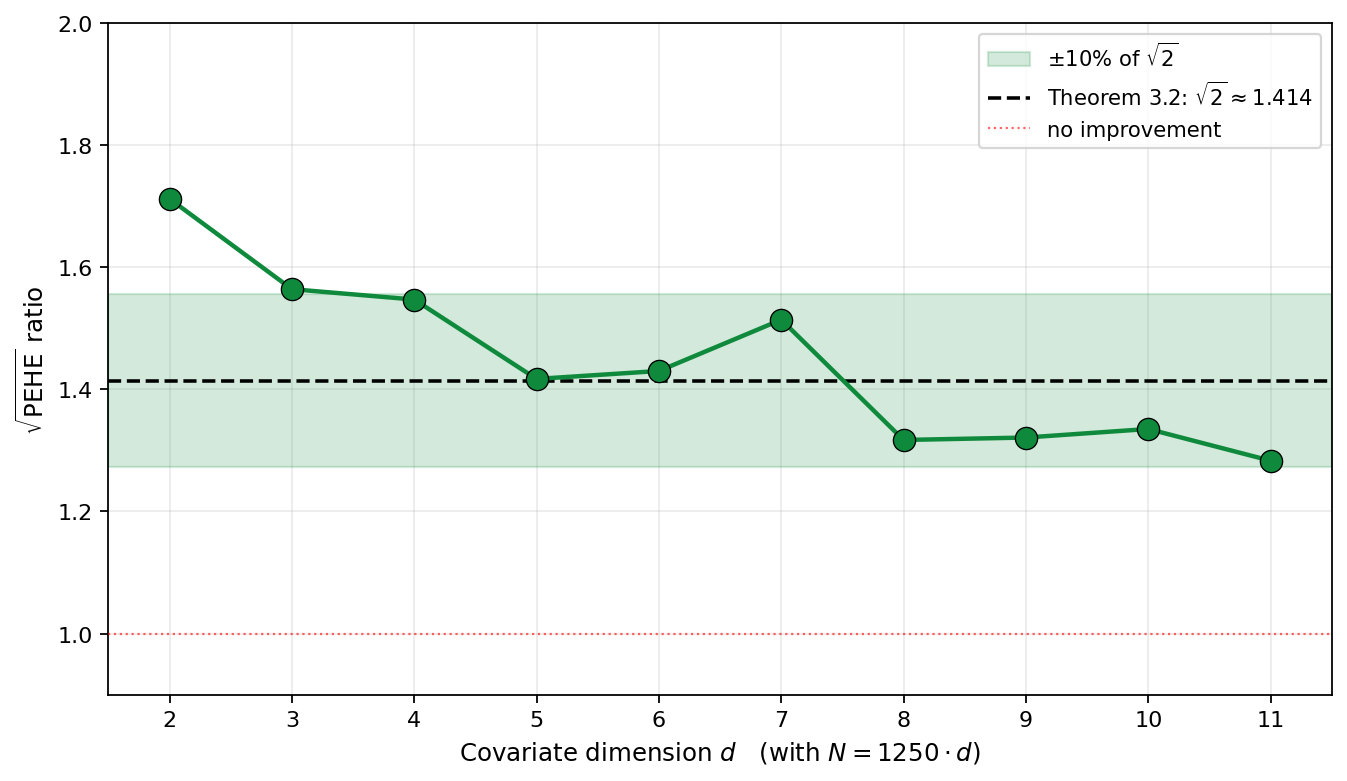
\includegraphics[width=0.72\textwidth]{d_scaling_law.png}
% \caption{$\sqrt{\mathrm{PEHE}}$ ratio at $N \approx 1250 \cdot d$ for
% $d = 2, \ldots, 11$ on the controlled linear SCM. Green line: per-cell
% mean over $K \geq 15$ SCMs. Shaded band: 95\% CI. Dashed line: Theorem
% \ref{thm:variance-ratio}'s prediction $\sqrt{2} \approx 1.414$.}
% \label{fig:d-scaling}
% \end{figure}

%----------------------------------------------------------------------
\section{MALC}
\label{app:malc}

Section~\ref{sec:cate-malc} recovers the per-unit CATE density by
marginalising a continuous joint density $\hat p(y_{0}, y_{1})$ fitted
to the joint-head grid $\{p_{j_{0}, j_{1}}\}$
of~\eqref{eq:pmat-softmax}. In this part we specify the details behind the estimator
used for $\hat p$: a $K$-component mixture of mean-adjusted log-concave
(MALC) densities, following the base construction of
\citet{danisman2026malc}. The mixture is needed because posteriors
over compatible SCMs can be multimodal, and a single
log-concave density is unimodal by construction; the shape constraint
is retained within each component while up to $K$ modes can be
represented across components.

\paragraph{Base class.}
Each mixture component is a single mean-adjusted log-concave (MALC)
density $\hat{f} \in \mathcal{F}_{\mathrm{LC}}$, where
$\mathcal{F}_{\mathrm{LC}}$ is the class of densities on
$\mathbb{R}^{2}$ with concave log. We take the constructor, sampling
proposal, and convergence guarantees of a single MALC fit as given by
\citet{danisman2026malc}. 

\paragraph{Mixture family.}
For a fixed order $K \geq 1$, the mixture family is
\begin{equation}
  \mathcal{F}_{\mathrm{MALC}}^{(K)}
  \;=\;
  \Big\{\,
    f \;=\; \sum_{k=1}^{K} \pi_{k}\, f_{k}
    \;:\;
    \pi \in \Delta^{K-1},\;\;
    f_{k} \in \mathcal{F}_{\mathrm{LC}}\;\;\forall k
  \,\Big\}.
  \label{eq:malc-family}
\end{equation}
Membership in $\mathcal{F}_{\mathrm{MALC}}^{(K)}$ permits up to $K$
modes while retaining the shape constraint componentwise.

\paragraph{Mixture EM on binned data.}
For $K > 1$, the components are combined by
expectation--maximisation directly on the grid. Let
$\gamma_{j_{0} j_{1}, k}^{(t)}$ denote the responsibility of component
$k$ for bin $(j_{0}, j_{1})$ at iteration $t$, and
$F_{k}^{(t)}(j_{0}, j_{1}) \coloneqq \int_{B_{j_{0}, j_{1}}}
f_{k}^{(t)}$ the bin-integrated component density. The updates are
\begin{align}
  \gamma_{j_{0} j_{1}, k}^{(t+1)}
  \;&=\;
  \frac{\pi_{k}^{(t)}\, F_{k}^{(t)}(j_{0}, j_{1})}
       {\sum_{l} \pi_{l}^{(t)}\, F_{l}^{(t)}(j_{0}, j_{1})},
  \label{eq:malc-estep}
  \\[2pt]
  \pi_{k}^{(t+1)}
  \;&=\;
  \sum_{j_{0}, j_{1}} p_{j_{0}, j_{1}}\, \gamma_{j_{0} j_{1}, k}^{(t+1)},
  \label{eq:malc-pi-update}
  \\[2pt]
  f_{k}^{(t+1)}
  \;&=\;
  \mathrm{MALC}\!\left(
    p_{j_{0}, j_{1}}\, \gamma_{j_{0} j_{1}, k}^{(t+1)}
  \right),
  \label{eq:malc-mstep}
\end{align}
Initialisation is a Voronoi assignment around the modal peaks of $p$, and the iterations stop after five consecutive non-improving log-likelihoods.

\paragraph{Order selection.}
The number of components is chosen by BIC on an effective sample size
$n_{\mathrm{eff}}$ derived from the grid probabilities themselves:
\begin{equation}
  n_{\mathrm{eff}}
  \;\coloneqq\;
  \Bigl(\sum_{j_{0}, j_{1}} p_{j_{0}, j_{1}}^{\, 2}\Bigr)^{-1},
  \qquad
  \mathrm{BIC}(K)
  \;=\;
  -2\, n_{\mathrm{eff}}\!
  \sum_{j_{0}, j_{1}} p_{j_{0}, j_{1}}\, \log \hat{f}^{(K)}(j_{0}, j_{1})
  \;+\;
  (3K - 1)\, \log n_{\mathrm{eff}},
  \label{eq:bic}
\end{equation}
where $\hat{f}^{(K)} \in \mathcal{F}_{\mathrm{MALC}}^{(K)}$ is the
mixture obtained by iterating
\eqref{eq:malc-estep}--\eqref{eq:malc-mstep} at order $K$. We select
$K^{\star} = \arg\min_{K \in \{1, \dots, K_{\max}\}} \mathrm{BIC}(K)$
with $K_{\max} = 5$. The parameter count $3K - 1$ tallies the $K - 1$
mixture weights plus a two-dimensional mean per component; the
log-concave shape itself does not contribute a finite parameter count.
The synthetic-sample size $B = 500$ is used inside each component
refit.

Each per-order fit is $\mathcal{O}(T \cdot K_{g}^{2} + T \cdot K \cdot
B \log B)$ where $T$ is the EM iteration count (typically $\leq 20$
in our experiments); the outer sweep over orders adds a factor
$K_{\max}$. Because the fit uses the binned probabilities directly, no
resampling of the original context is required and the whole
procedure runs on a single CPU per query.

\paragraph{Output and downstream use.}
The MALC estimator is a smooth density
\begin{equation}
  \hat{p}_{\mathrm{MALC}}(y_{0}, y_{1})
  \;=\;
  \sum_{k=1}^{K^{\star}} \hat{\pi}_{k}^{\star}\,
  \hat{f}_{k}^{\star}(y_{0}, y_{1})
  \label{eq:malc-output}
\end{equation}
on the convex hull of the synthetic points that generated the
components, evaluable at any query $(y_{0}, y_{1}) \in \mathbb{R}^{2}$.

%----------------------------------------------------------------------
\section{Optimal-transport aggregation}
\label{app:ot}

Section~\ref{sec:ate-barycenter} defines the ATE density
$f_{\mathrm{ATE}}$ as the uniformly-weighted 2-Wasserstein barycenter
of the per-query CATE densities $\{f_{\tau}^{(n)}\}_{n=1}^{N}$ and
states its closed-form quantile representation
in~\eqref{eq:ate-quantile}. In this segment we report the derivation and the
grid-level algorithm used for ATE.

\paragraph{Notation.}
Let $F_{n}$ and $Q_{n} \coloneqq F_{n}^{-1}$ be the CDF and quantile
function of the per-query CATE density $f_{\tau}^{(n)}$, and let
$\alpha \in \Delta^{N-1}$ be nonnegative weights summing to $1$. On
$\mathbb{R}$ the weighted 2-Wasserstein barycenter of
$\{f_{\tau}^{(n)}\}_{n=1}^{N}$ admits the closed-form quantile
representation
\begin{equation}
  Q^{\star}(t)
  \;=\;
  \sum_{n=1}^{N} \alpha_{n}\, Q_{n}(t),
  \qquad
  t \in (0, 1),
  \label{eq:agueh-carlier}
\end{equation}
of which~\eqref{eq:ate-quantile} is the uniform-weight case $\alpha_{n} = 1/N$.

\paragraph{Grid-level implementation.}
Because $Q^{\star}$ is defined explicitly by~\eqref{eq:agueh-carlier},
no iterative optimisation is needed. Given the per-query densities
sampled on a common grid $x_{1} < \cdots < x_{M}$ with spacing
$\Delta x$, the barycenter density is produced in three quantile
passes and one density-recovery pass:
\begin{enumerate}[label=\arabic*., leftmargin=1.8em]
  \item Discretise the probability axis by $\tau_{j} \coloneqq
    (j - \tfrac{1}{2}) / M_{\tau}$ for $j = 1, \dots, M_{\tau}$
    (we use $M_{\tau} = 4001$).
  \item For each query $n \in \{1, \dots, N\}$, compute the CDF by
    trapezoidal integration, renormalise, and invert to obtain the
    quantile function at every $\tau_{j}$:
    \[
      F_{n}(x_{k}) \;\gets\;
        \sum_{\ell \leq k}
        \tfrac{1}{2}\bigl(\hat{p}_{n}(x_{\ell - 1})
        + \hat{p}_{n}(x_{\ell})\bigr)\, \Delta x,
      \quad
      F_{n} \;\gets\; F_{n} / F_{n}(x_{M}),
      \quad
      Q_{n}(\tau_{j}) \;\gets\; F_{n}^{-1}(\tau_{j}).
    \]
  \item Average the quantile functions pointwise per
    \eqref{eq:agueh-carlier}: $Q^{\star}(\tau_{j}) = \sum_{n}
    \alpha_{n}\, Q_{n}(\tau_{j})$.
  \item Recover the barycenter density on the original grid: invert
    $Q^{\star}$ back to a CDF $F^{\star}$, take a central-difference
    derivative, and renormalise to unit integral,
    \[
      \hat{f}_{\mathrm{ATE}}(x_{k}) \;\gets\;
        \frac{F^{\star}(x_{k+1}) - F^{\star}(x_{k-1})}{2\, \Delta x},
      \qquad
      \hat{f}_{\mathrm{ATE}} \;\gets\; \hat{f}_{\mathrm{ATE}} \Big/
        \Bigl(\Delta x \sum_{k} \hat{f}_{\mathrm{ATE}}(x_{k})\Bigr).
    \]
\end{enumerate}
Every step is $\mathcal{O}(N \cdot M)$ vector arithmetic; producing
$\hat{f}_{\mathrm{ATE}}$ is therefore much cheaper than the per-query
MALC fits it aggregates.




\section{Theory Validation something something}
\label{app:theoryval}


%======================================================================
\bibliographystyle{plainnat}
\begin{thebibliography}{9}

\bibitem[van~der~Vaart(1998)]{van-der-vaart-1998-asymptotic-statistics}
A.~W.\ van~der~Vaart.
\newblock \emph{Asymptotic Statistics}.
\newblock Cambridge University Press, 1998.

\bibitem[Sheppard(1899)]{sheppard1899application}
W.~F.\ Sheppard.
\newblock On the application of the theory of error to cases of normal distribution and normal correlation.
\newblock \emph{Philosophical Transactions of the Royal Society A}, 192:101--167, 1899.

\bibitem[Danisman(2026)]{danisman2026malc}
F.~Danisman.
\newblock Mean-adjusted log-concave density estimation, 2026. Working paper.

\end{thebibliography}

\end{document}
